% Exemplos de uso do LATEX

\chapter*{Resumo \label{resumo}}

\section{Objetivo \label{objetivo}}

\subsection{Objetivo \label{objetivo}}

\begin{figure}[h|top]
 \centering
 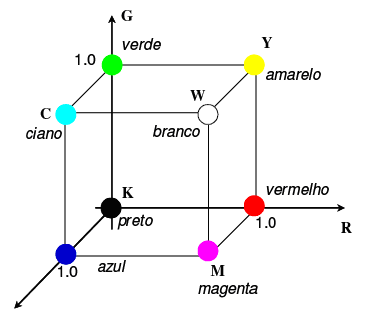
\includegraphics[width=0.7\linewidth]{imagens/rgb.png}
 \caption{Sistema RGB.}
 \label{img_rgb}
\end{figure}

\begin{table}[htb] % [htb]-> here, top, botton
   \centering   % tabela centralizada
   \large       % tamanho da fonte
   \setlength{\arrayrulewidth}{2\arrayrulewidth}  % espessura da  linha
   \setlength{\belowcaptionskip}{10pt}  % espa�o entre caption e tabela
   \caption{\it Tabela com algumas das muitas combina��es de cores poss�veis com o sistema RGB.}
   \begin{tabular}{|l|c|c|c|} % c=center, l=left, r=right

        \hline Cor & R & G & B \\
        \hline Preto & 0 & 0 &  0 \\
        \hline Preto Escuro & 0 & 0 & 128 \\
        \hline Azul & 0 & 0 & 255 \\
        \hline Verde Escuro & 0 & 128 & 0 \\
        \hline Turquesa & 0 & 128& 128 \\
        \hline Azul Claro &0 &128 &255 \\
        \hline Verde & 0 & 255 & 0 \\
        \hline Verde �gua & 0 & 255 & 128 \\
        \hline Ciano & 0 & 255 & 255 \\
        \hline Marrom & 128 & 0 & 0 \\
        \hline Violeta & 128 & 0 & 128 \\
        \hline Azul Marinho & 128 & 0 & 255 \\
        \hline Verde Musgo & 128 & 128 & 0 \\
        \hline Cinza & 128 & 128 & 128 \\
        \hline

   \end{tabular}
   \label{tab:rgb}
\end{table}

\begin{large}
\begin{center}
\begin{equation}
\label{eq:label}
$ND = \sum_{i=n}^{n}{MiOi}$
\end{equation}
\end{center}
\end{large}

